% Options for packages loaded elsewhere
\PassOptionsToPackage{unicode}{hyperref}
\PassOptionsToPackage{hyphens}{url}
%
\documentclass[
]{book}
\usepackage{amsmath,amssymb}
\usepackage{lmodern}
\usepackage{iftex}
\ifPDFTeX
  \usepackage[T1]{fontenc}
  \usepackage[utf8]{inputenc}
  \usepackage{textcomp} % provide euro and other symbols
\else % if luatex or xetex
  \usepackage{unicode-math}
  \defaultfontfeatures{Scale=MatchLowercase}
  \defaultfontfeatures[\rmfamily]{Ligatures=TeX,Scale=1}
\fi
% Use upquote if available, for straight quotes in verbatim environments
\IfFileExists{upquote.sty}{\usepackage{upquote}}{}
\IfFileExists{microtype.sty}{% use microtype if available
  \usepackage[]{microtype}
  \UseMicrotypeSet[protrusion]{basicmath} % disable protrusion for tt fonts
}{}
\makeatletter
\@ifundefined{KOMAClassName}{% if non-KOMA class
  \IfFileExists{parskip.sty}{%
    \usepackage{parskip}
  }{% else
    \setlength{\parindent}{0pt}
    \setlength{\parskip}{6pt plus 2pt minus 1pt}}
}{% if KOMA class
  \KOMAoptions{parskip=half}}
\makeatother
\usepackage{xcolor}
\usepackage{longtable,booktabs,array}
\usepackage{calc} % for calculating minipage widths
% Correct order of tables after \paragraph or \subparagraph
\usepackage{etoolbox}
\makeatletter
\patchcmd\longtable{\par}{\if@noskipsec\mbox{}\fi\par}{}{}
\makeatother
% Allow footnotes in longtable head/foot
\IfFileExists{footnotehyper.sty}{\usepackage{footnotehyper}}{\usepackage{footnote}}
\makesavenoteenv{longtable}
\usepackage{graphicx}
\makeatletter
\def\maxwidth{\ifdim\Gin@nat@width>\linewidth\linewidth\else\Gin@nat@width\fi}
\def\maxheight{\ifdim\Gin@nat@height>\textheight\textheight\else\Gin@nat@height\fi}
\makeatother
% Scale images if necessary, so that they will not overflow the page
% margins by default, and it is still possible to overwrite the defaults
% using explicit options in \includegraphics[width, height, ...]{}
\setkeys{Gin}{width=\maxwidth,height=\maxheight,keepaspectratio}
% Set default figure placement to htbp
\makeatletter
\def\fps@figure{htbp}
\makeatother
\setlength{\emergencystretch}{3em} % prevent overfull lines
\providecommand{\tightlist}{%
  \setlength{\itemsep}{0pt}\setlength{\parskip}{0pt}}
\setcounter{secnumdepth}{5}
\usepackage{booktabs}
\ifLuaTeX
  \usepackage{selnolig}  % disable illegal ligatures
\fi
\usepackage[]{natbib}
\bibliographystyle{plainnat}
\IfFileExists{bookmark.sty}{\usepackage{bookmark}}{\usepackage{hyperref}}
\IfFileExists{xurl.sty}{\usepackage{xurl}}{} % add URL line breaks if available
\urlstyle{same} % disable monospaced font for URLs
\hypersetup{
  pdftitle={BIOSTATS},
  pdfauthor={Akira Terui},
  hidelinks,
  pdfcreator={LaTeX via pandoc}}

\title{BIOSTATS}
\author{Akira Terui}
\date{Last updated on 2022-09-14}

\begin{document}
\maketitle

{
\setcounter{tocdepth}{1}
\tableofcontents
}
\hypertarget{introduction}{%
\chapter{Introduction}\label{introduction}}

This textbook aims to introduce fundamental statistical techniques and their applications to biological data. A unique aspect of this book is the ``flipped-order'' introduction. Many statistics courses start with theory; yet, I found it difficult for those unfamiliar with statistics. I will start with a real example of the method, followed by an explanation for an underlying theory/concept. The author is an ecologist, so some methods in this book might not be popular in other fields.

\hypertarget{project-management}{%
\chapter{Project Management}\label{project-management}}

\hypertarget{r-project}{%
\section{R Project}\label{r-project}}

For this entire book, I will use \texttt{R\ Project} as a fundamental unit of work-space, in which all the relevant materials (e.g., R scripts \texttt{.R} and data files) are assembled together. There are many ways to organize your project, but I usually make a single \texttt{R\ Project} for a collection of scripts and data that will lead to a single publication (see example \href{https://github.com/aterui/public-proj_stream-diversity}{here}). To setup an \texttt{R\ Project} you will need \emph{R Studio} in addition to base \emph{R}. While \emph{R} is a stand-alone software, I strongly recommend to use it with \emph{R Studio}. \emph{R Studio} has many functions that help your data analysis. \emph{R} and \emph{R Studio} can be installed from the following websites:

\begin{itemize}
\tightlist
\item
  \href{https://www.r-project.org/}{R} (you can choose any CRAN mirror to download)
\item
  \href{https://rStudio.com/products/rStudio/download/}{R Studio}
\end{itemize}

Once you open \emph{R Studio}, you will see the following interface (Figure \ref{fig:ui}). There are three major panels in its first appearance -- \texttt{Console}, \texttt{Environment}, and \texttt{Files}. \texttt{Console} is the place where you write your codes and execute calculation/data manipulation/analysis. \texttt{Environment} lists items you saved as an object. \texttt{Files} list any files in a designated location in your computer.

\begin{figure}
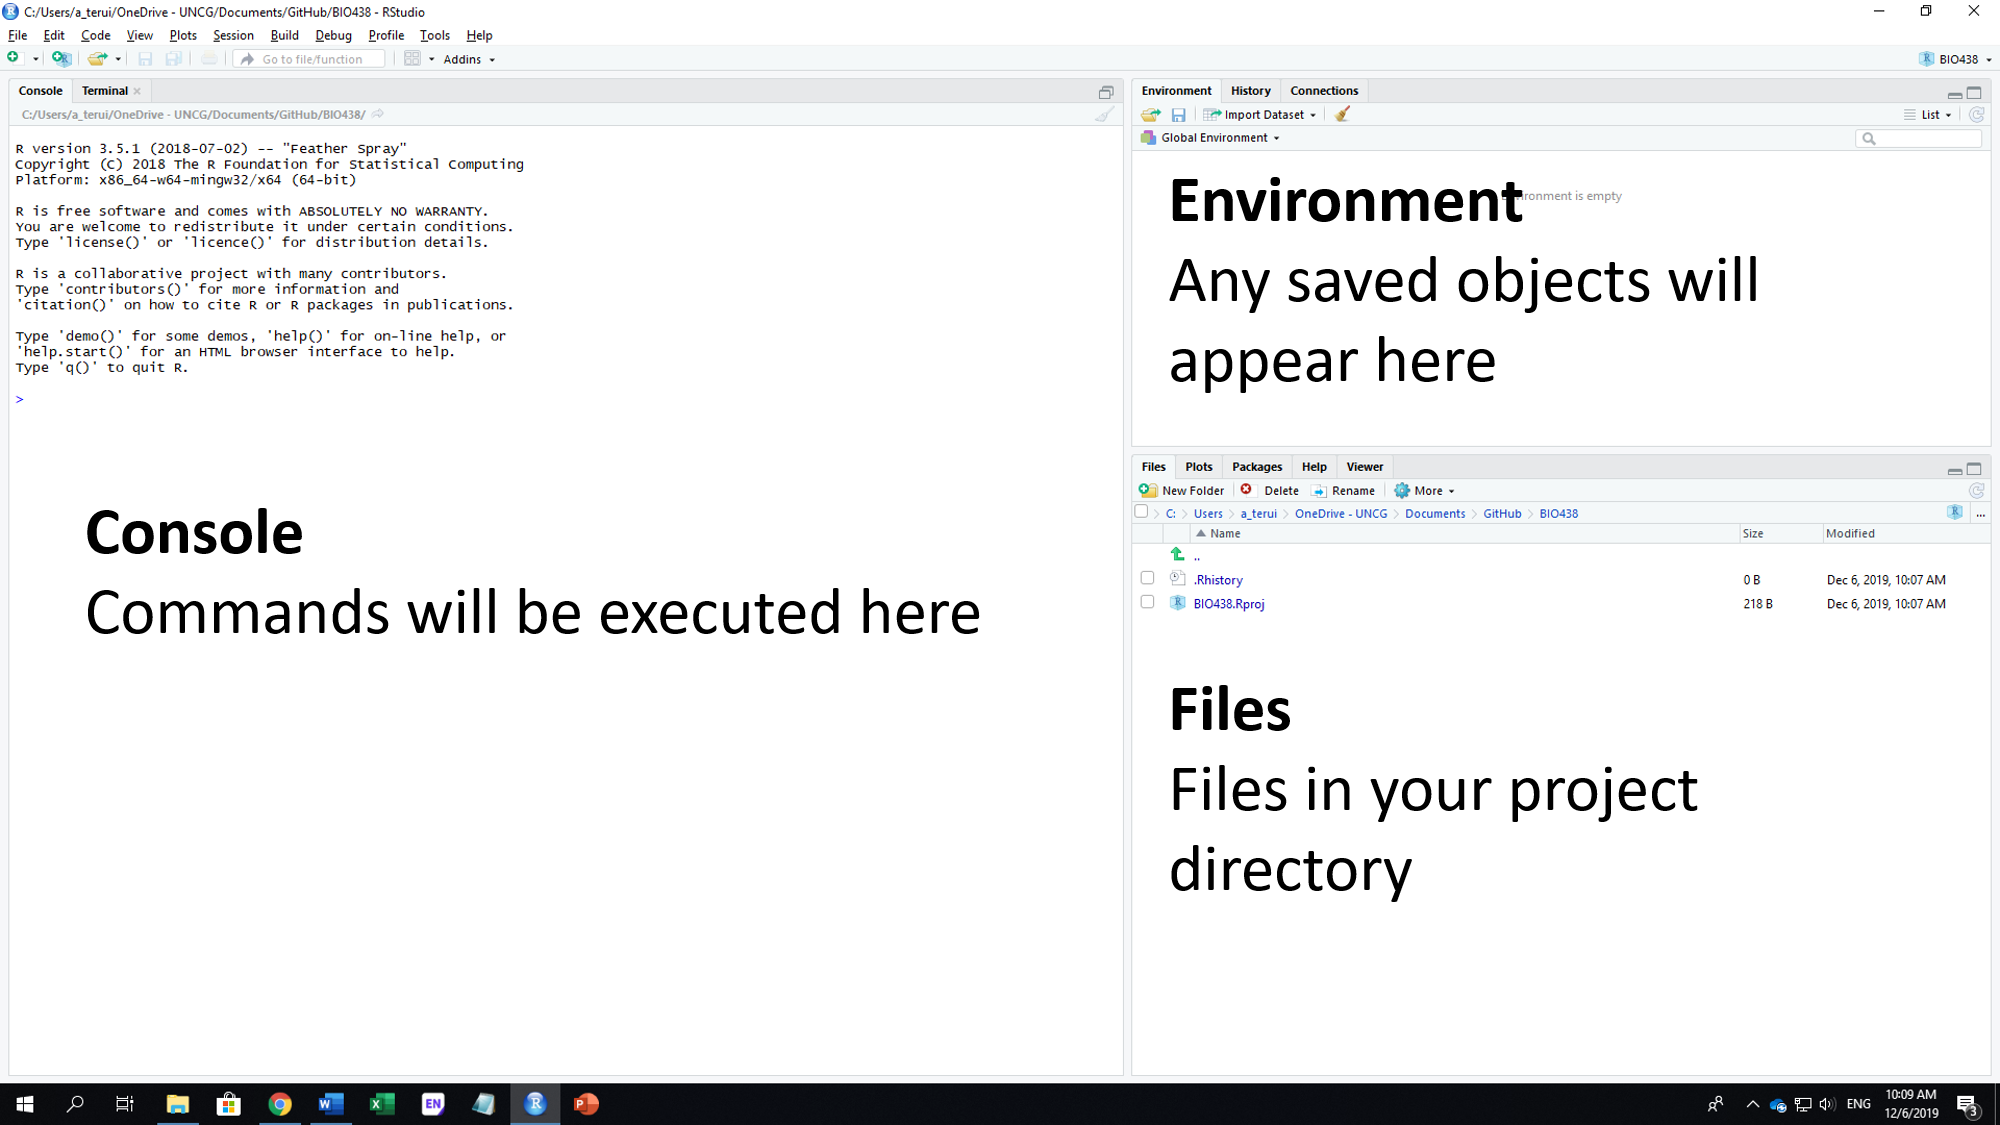
\includegraphics[width=27.78in]{image/r_image01} \caption{R Studio interface.}\label{fig:ui}
\end{figure}

Although you can work on your data as it appears, \textbf{it is actually a BAD idea}. As you work on your project, numerous materials will be generated. How do you manage files? If you randomly locate those materials within your computer, you will lose necessary items sooner or later. For this reason, I assemble all the relevant materials in a single \texttt{R\ Project}. You can create a new \texttt{R\ Project} with the following procedure.

\begin{enumerate}
\def\labelenumi{\alph{enumi}.}
\tightlist
\item
  Go to \texttt{File\ \textgreater{}\ New\ Project} on the top menu
\item
  Select \texttt{New\ Directory}
\item
  Select \texttt{New\ Project}
\end{enumerate}

A new window pops up and prompts you to name a directory with a location in your computer. Click \texttt{Browse} to select a location for the directory.

\textbf{IMPORTANT:} When you locate your project directories in your computer, I would strongly recommend to create a designated space. For example, in my computer, I have a folder named /\texttt{r\_project} in which all the \texttt{R\ Project} directories are located.

\hypertarget{internal-structure}{%
\section{Internal Structure}\label{internal-structure}}

The internal structure of an \texttt{R\ Project} is extremely important to navigate yourself (others once it's published). \texttt{R\ Project} will be composed of multiple types of files, typically \texttt{.R}, \texttt{.csv}, \texttt{.rds}, \texttt{.Rmd} among others. Unless those files are arranged in an organized manner, it is VERY LIKELY to make severe errors in coding. So I take this seriously. Table \ref{tab:str} is my suggested subdirectory structure.

\begin{longtable}[]{@{}
  >{\raggedright\arraybackslash}p{(\columnwidth - 2\tabcolsep) * \real{0.0838}}
  >{\raggedright\arraybackslash}p{(\columnwidth - 2\tabcolsep) * \real{0.9162}}@{}}
\caption{\label{tab:str} Suggested internal structure of \texttt{R\ Project}}\tabularnewline
\toprule()
\begin{minipage}[b]{\linewidth}\raggedright
Name
\end{minipage} & \begin{minipage}[b]{\linewidth}\raggedright
Content
\end{minipage} \\
\midrule()
\endfirsthead
\toprule()
\begin{minipage}[b]{\linewidth}\raggedright
Name
\end{minipage} & \begin{minipage}[b]{\linewidth}\raggedright
Content
\end{minipage} \\
\midrule()
\endhead
\texttt{README.md} & Markdown file explaining contents in the \texttt{R\ Project}. Can be derived from \texttt{README.Rmd}. \\
\texttt{/code} & Sub-directory for R scripts (\texttt{.R}). \\
\texttt{/data\_raw} & Sub-directory for raw data before data manipulation (\texttt{.csv} or other formats). Files in this sub-directory MUST NOT be modified unless there are changes to raw data entries. \\
\texttt{/data\_format} & Sub-directory for formatted data (\texttt{.csv}, \texttt{.rds}, or other formats). \\
\texttt{/output} & Sub-directory for result outputs (\texttt{.csv}, \texttt{.rds}, or other formats). This may include statistical estimates from linear regression models etc. \\
\texttt{/rmd} & (Optional) Sub-directory for Rmarkdown files (\texttt{.Rmd}). Rmarkdown allows seamless integration of R scripts and text. \\
\bottomrule()
\end{longtable}

It is also critical to have \textbf{consistent naming rules} for your files. As you make progress on your project, the number of files in each sub-directory will increase, perhaps exponentially. You will find it difficult navigating yourself unless you have clear naming rules for files (and even worse for others). Here are some recommendations:

\begin{itemize}
\tightlist
\item
  \textbf{NO SPACE.} Instead, use underscore.

  \begin{itemize}
  \tightlist
  \item
    Do: \texttt{script\_week1.R}
  \item
    Don't: \texttt{script\ week1.R}
  \end{itemize}
\item
  \textbf{NO UPPERCASE.} Use lowercase for file names.

  \begin{itemize}
  \tightlist
  \item
    Do: \texttt{script\_week1.R}
  \item
    Don't: \texttt{Script\_week1.R}
  \end{itemize}
\item
  \textbf{BE CONSISTENT.} Apply consistent naming rules within a project.

  \begin{itemize}
  \tightlist
  \item
    Do: R scripts for figures always start with a common prefix, e.g., \texttt{figure\_XXX.R} \texttt{figure\_YYY.R}(\texttt{XXX} and \texttt{YYY} specifies further details).
  \item
    Don't: R scripts for figures start with random text, e.g., \texttt{XXX\_fig.R} , \texttt{Figure\_Y2.R} , \texttt{plotB.R}.
  \end{itemize}
\end{itemize}

  \bibliography{book.bib,packages.bib}

\end{document}
